\documentclass[aspectratio=169]{beamer}
\usetheme{Madrid}
\usecolortheme{default}

% ── Packages ──────────────────────────────────────────────────────────────────
\usepackage{amsmath, amssymb}
\usepackage{graphicx}
\usepackage{booktabs}
\usepackage{colortbl}
\usepackage{xcolor}
\usepackage{tikz}
\usepackage{pgfplots}
\pgfplotsset{compat=1.18}

% ── Color palette ─────────────────────────────────────────────────────────────
\definecolor{madridblue}{RGB}{0,60,120}
\definecolor{accentred}{RGB}{180,30,30}
\setbeamercolor{alerted text}{fg=accentred}

% ── Title info ────────────────────────────────────────────────────────────────
\title[Mortgage Prepayment \& Credit Risk]{%
  Mortgage Prepayment and Credit Risk Modeling}
\subtitle{MTH9877 — Interest Rate and Credit Models}
\author{Yueqi Lin}
\institute{Baruch College, CUNY}
\date{May 13, 2026}

\setbeamertemplate{footline}[frame number]

% ══════════════════════════════════════════════════════════════════════════════
\begin{document}

\begin{frame}
  \titlepage
\end{frame}

\begin{frame}{Outline}
  \tableofcontents[hideallsubsections]
\end{frame}

% ══════════════════════════════════════════════════════════════════════════════
\section{Motivation \& Data}

\begin{frame}{Mortgages as Survival Problems}
  \begin{columns}
    \column{0.55\textwidth}
      \textbf{Key modeling challenge:} two competing termination risks
      \begin{itemize}
        \item \alert{Prepayment} — refinancing or home sale
        \item \alert{Default} — borrower stops paying
      \end{itemize}
      \vspace{0.4em}
      Both are \textbf{time-to-event} phenomena driven by:
      \begin{itemize}
        \item Loan characteristics (LTV, FICO, coupon)
        \item Borrower profile (DTI, loan purpose)
        \item Macro environment (rates, HPI, unemployment)
      \end{itemize}
      \vspace{0.4em}
      \textbf{Goal:} estimate and interpret hazard rates using survival
      analysis, ML, and deep learning.
    \column{0.42\textwidth}
      \begin{block}{Why it matters}
        MBS pricing, hedging, and duration management all depend on
        accurate prepayment models.
        A 1\% CPR error can shift OAS by 20–50 bp.
      \end{block}
  \end{columns}
\end{frame}

\begin{frame}{Dataset — Freddie Mac Single-Family Loans}
  \begin{columns}
    \column{0.48\textwidth}
      \textbf{Source:} Freddie Mac CRT loan-level data (1999–2025)\\[0.4em]
      \textbf{Filter:} 30-year FRM only
      \begin{table}
        \small
        \begin{tabular}{lr}
          \toprule
          \textbf{} & \textbf{Count} \\
          \midrule
          Total FRM-360 loans & 34.0M \\
          Prepaid (ZBC = 1)   & 21.97M~~(64.6\%) \\
          Defaulted (ZBC 2/3/9) & 0.53M~~(1.6\%) \\
          Censored (active)   & 11.51M~~(33.8\%) \\
          \midrule
          Median duration     & 32 months \\
          FICO (mean)         & 742 \\
          LTV (mean)          & 74.4 \\
          Coupon (mean)       & 5.06\% \\
          \bottomrule
        \end{tabular}
      \end{table}
    \column{0.48\textwidth}
      \textbf{Static loan features}
      \begin{itemize}\small
        \item FICO, LTV, DTI, original rate, UPB
        \item Loan purpose (P/C/N), Occupancy, State
        \item Origination vintage (1999–2025)
      \end{itemize}
      \vspace{0.3em}
      \textbf{Macro covariates (FRED, monthly)}
      \begin{itemize}\small
        \item 30-yr mortgage rate (\texttt{MORTGAGE30US})
        \item Unemployment rate (\texttt{UNRATE})
        \item CPI YoY inflation (\texttt{CPIAUCSL})
        \item Case-Shiller HPI YoY (\texttt{CSUSHPISA})
      \end{itemize}
      \vspace{0.3em}
      \textbf{Key engineered feature:}\\
      Rate incentive $= r^{\text{orig}} - r^{\text{mkt}}_t$
  \end{columns}
\end{frame}

% ══════════════════════════════════════════════════════════════════════════════
\section{Part A: Exploratory Survival Analysis}

\begin{frame}{Kaplan-Meier Survival Curve \& Hazard Rate}
  \begin{columns}
    \column{0.52\textwidth}
      \begin{figure}
        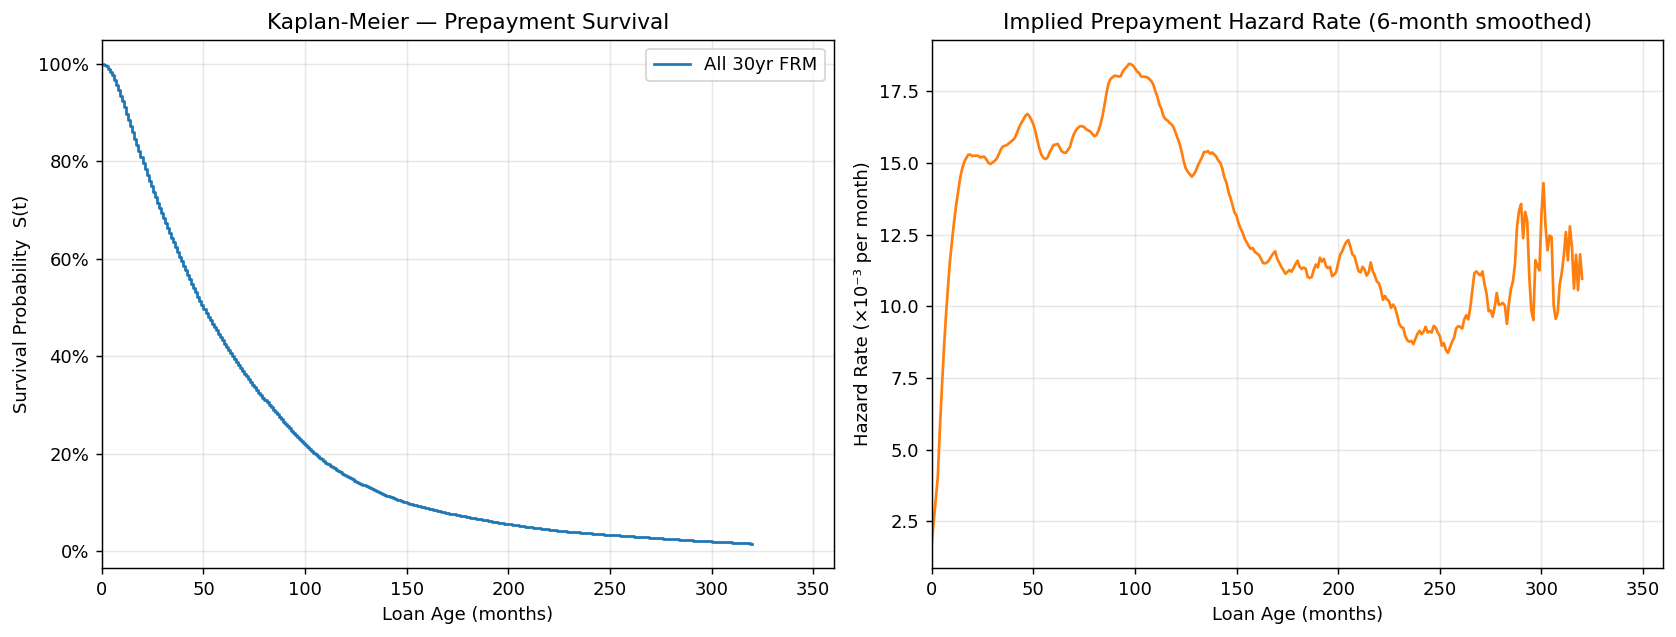
\includegraphics[width=\linewidth]{processed/A1_km_hazard.png}
      \end{figure}
    \column{0.44\textwidth}
      \textbf{Key observations:}
      \begin{itemize}
        \item \textbf{Median prepayment time: 32 months}
        \item Hazard rate peaks around months 24–48 (seasoning hump)
        \item Consistent with the PSA ramp-up period
        \item $\sim$35\% of loans survive beyond 100 months (burnout effect)
        \item Hazard declines after 60 months — seasoned borrowers are rate-insensitive
      \end{itemize}
      \vspace{0.3em}
      \begin{block}{Burnout}
        Rate-sensitive borrowers prepay early; those who remain are
        less likely to refinance even when rates fall.
      \end{block}
  \end{columns}
\end{frame}

\begin{frame}{Stratified Kaplan-Meier Curves}
  \begin{columns}
    \column{0.32\textwidth}
      \begin{figure}
        \centering
        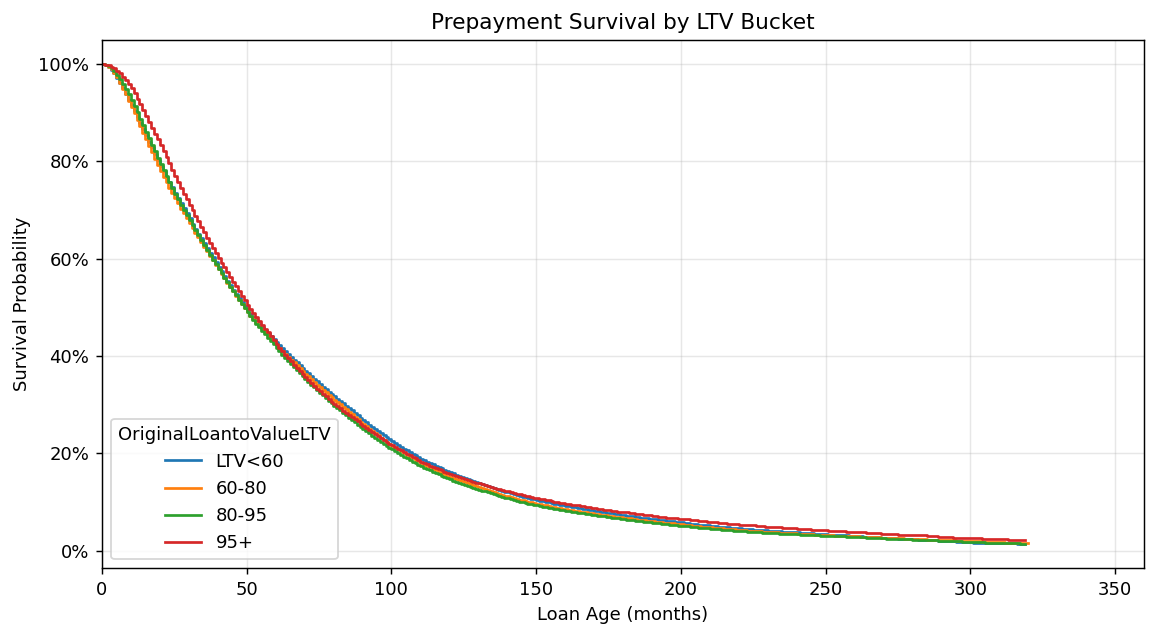
\includegraphics[width=\linewidth]{processed/A2_km_ltv.png}
        \caption{\small By LTV bucket}
      \end{figure}
    \column{0.32\textwidth}
      \begin{figure}
        \centering
        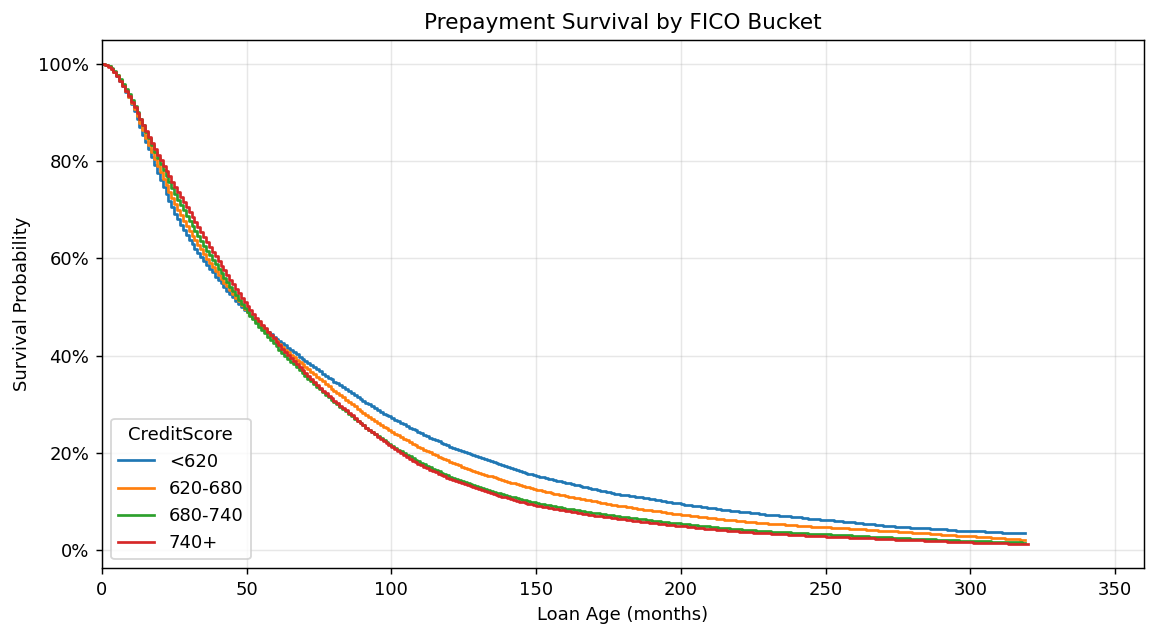
\includegraphics[width=\linewidth]{processed/A2_km_fico.png}
        \caption{\small By FICO bucket}
      \end{figure}
    \column{0.32\textwidth}
      \begin{figure}
        \centering
        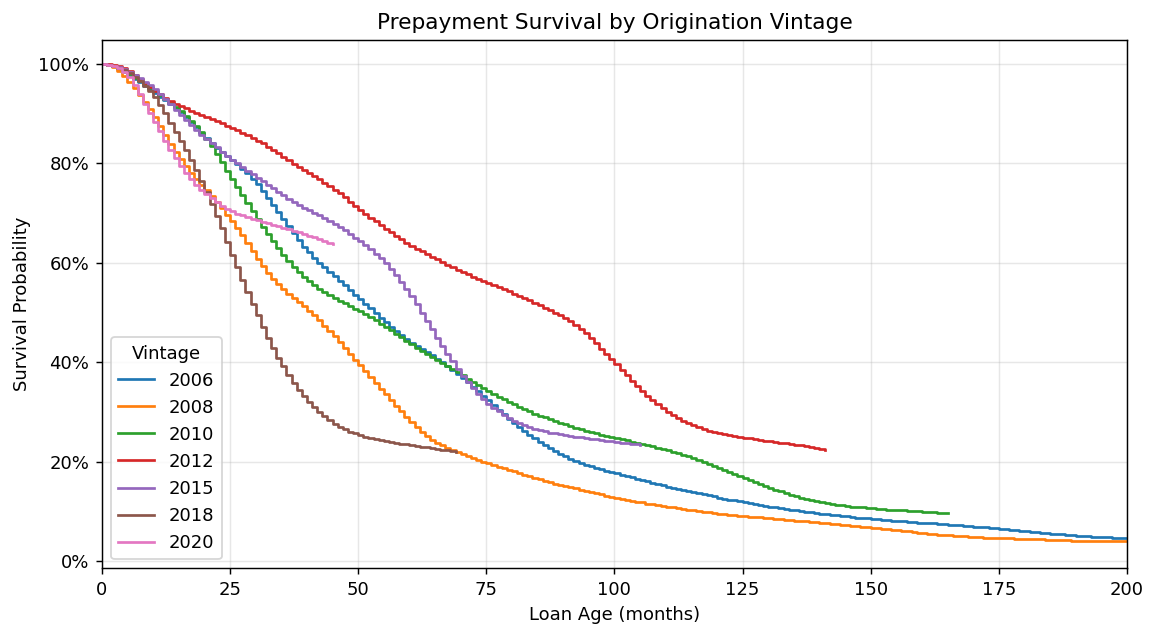
\includegraphics[width=\linewidth]{processed/A2_km_vintage.png}
        \caption{\small By origination vintage}
      \end{figure}
  \end{columns}
  \vspace{0.2em}
  \small
  \textbf{LTV:} Low-LTV loans prepay faster — more equity enables refinancing.~~
  \textbf{FICO:} Higher-credit borrowers have better capital market access.~~
  \textbf{Vintage 2020–21:} Historic rate lows triggered the fastest prepayment wave on record.
\end{frame}

% ══════════════════════════════════════════════════════════════════════════════
\section{Part B: Cox Proportional Hazards Model}

\begin{frame}{Cox PH Model — Hazard Ratios}
  \begin{columns}
    \column{0.50\textwidth}
      \begin{figure}
        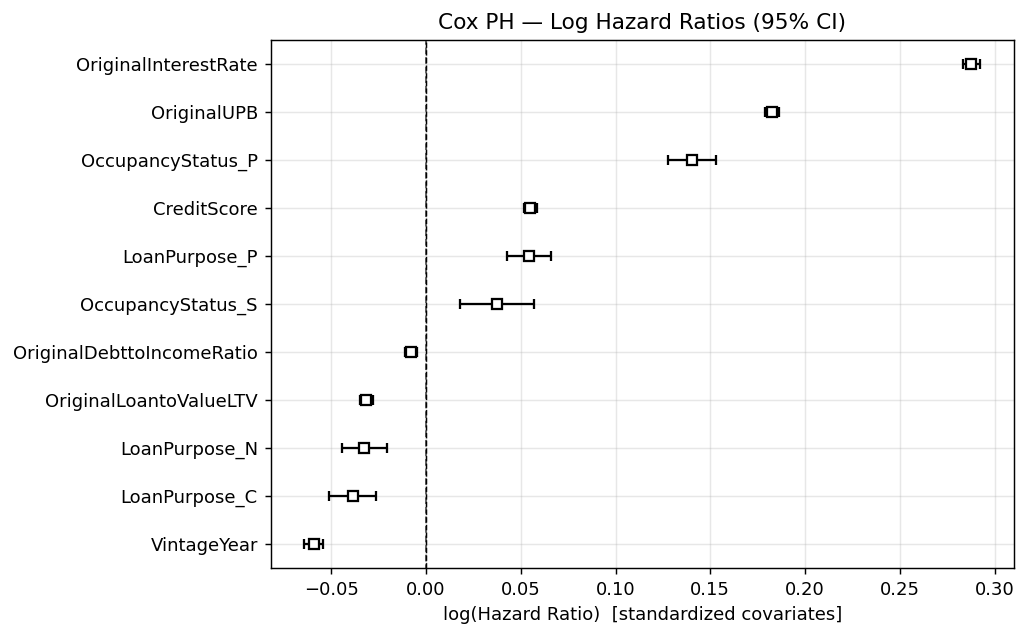
\includegraphics[width=\linewidth]{processed/B1_cox_hr.png}
      \end{figure}
    \column{0.46\textwidth}
      \small
      \begin{tabular}{lcc}
        \toprule
        \textbf{Covariate} & \textbf{HR} & \textbf{Direction} \\
        \midrule
        FICO (std.)         & 1.057 & $\uparrow$ prepay \\
        LTV (std.)          & 0.969 & $\downarrow$ prepay \\
        Original rate (std.)& 1.333 & $\uparrow$ prepay \\
        DTI (std.)          & 0.992 & $\downarrow$ prepay \\
        UPB (std.)          & 1.200 & $\uparrow$ prepay \\
        Vintage year        & 0.943 & $\downarrow$ prepay \\
        \bottomrule
      \end{tabular}
      \vspace{0.4em}
      \begin{itemize}
        \item Original rate HR = \textbf{1.33}: high-coupon loans have
          the strongest refi incentive
        \item LTV HR = \textbf{0.97}: underwater borrowers cannot refinance
        \item \textbf{C-index = 0.611}
      \end{itemize}
  \end{columns}
\end{frame}

\begin{frame}{PH Assumption Test — Schoenfeld Residuals}
  \begin{columns}
    \column{0.54\textwidth}
      \begin{figure}
        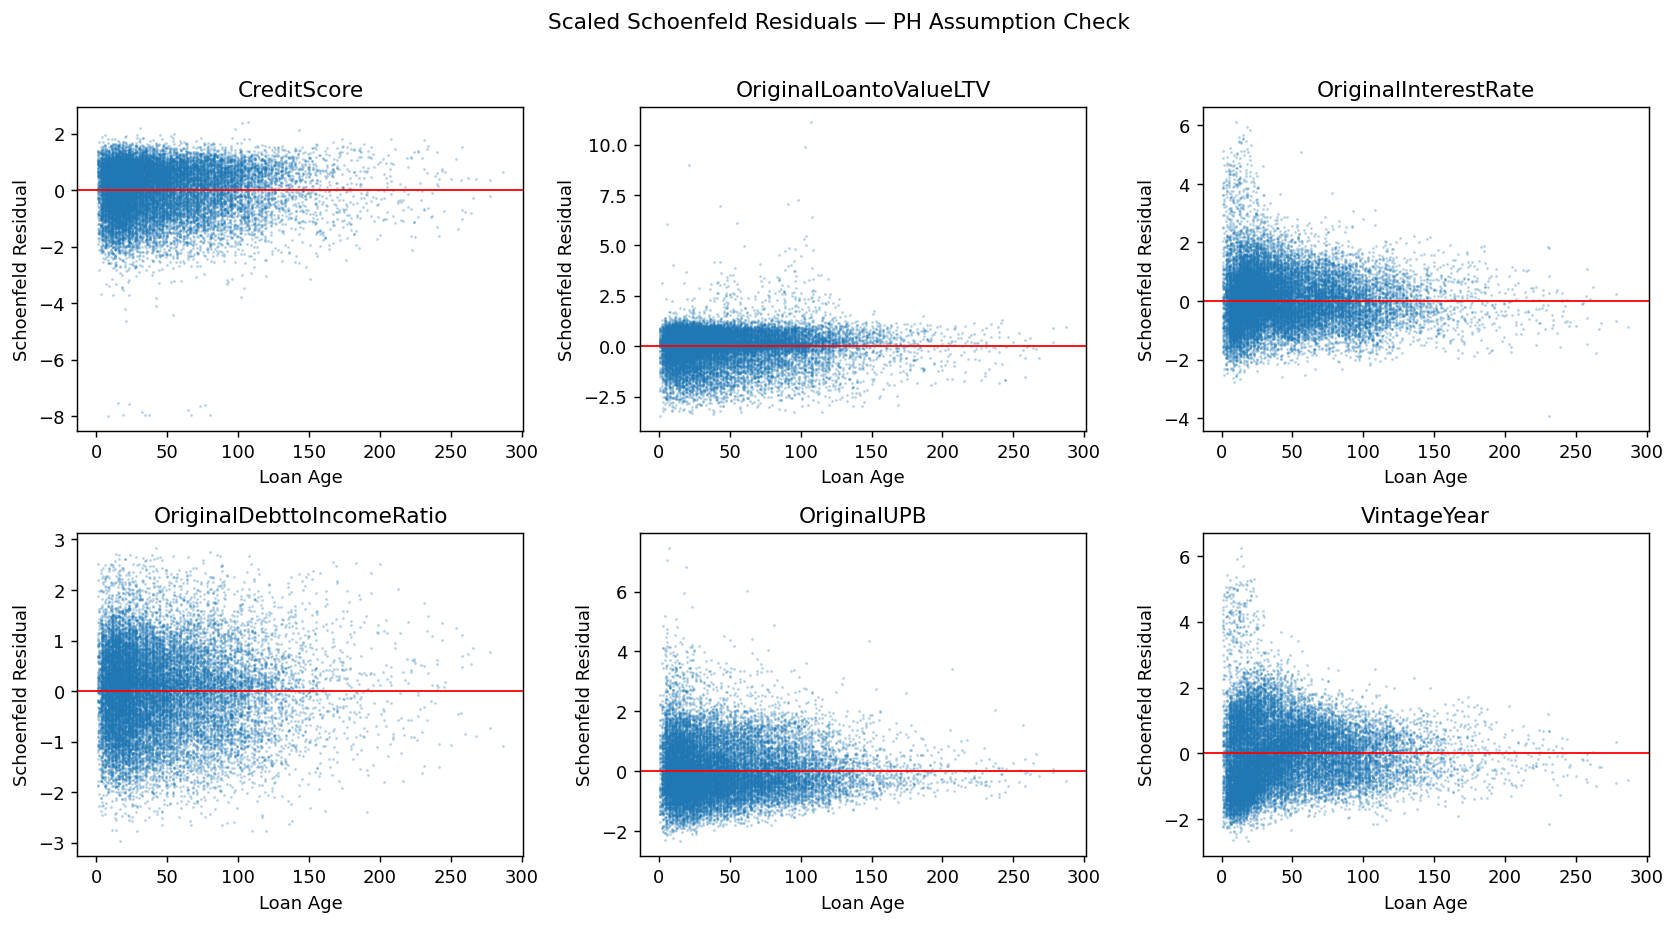
\includegraphics[width=\linewidth]{processed/B2_schoenfeld.png}
      \end{figure}
    \column{0.42\textwidth}
      \textbf{All key covariates violate PH} (p $\ll$ 0.001):
      \begin{itemize}\small
        \item \texttt{OriginalInterestRate}: $\chi^2 = 728$,
          $p = 2.3 \times 10^{-160}$
        \item \texttt{LTV}: $\chi^2 = 290$, $p = 6.2 \times 10^{-65}$
        \item \texttt{FICO}: $\chi^2 = 160$, $p = 1.0 \times 10^{-36}$
      \end{itemize}
      \vspace{0.3em}
      Only \texttt{OccupancyStatus\_S} does not violate ($p = 0.90$).
      \begin{alertblock}{Implication}
        The proportional hazards assumption fails — covariate
        effects \emph{change} with loan age. This motivates
        time-varying covariates and nonlinear models.
      \end{alertblock}
  \end{columns}
\end{frame}

\begin{frame}{Time-Varying Cox with Macro Covariates}
  \[
    \lambda(t \mid \mathbf{x}(t)) = \lambda_0(t)\,\exp\!\bigl(
      \underbrace{0.033\,\Delta r_t}_{\text{rate incentive}}
      - 0.017\,r^{\text{mkt}}_t
      + 0.012\,u_t
      - 0.007\,\pi_t
      + 0.003\,h_t + \cdots\bigr)
  \]
  \begin{columns}
    \column{0.48\textwidth}
      \textbf{Key findings:}
      \begin{itemize}
        \item \alert{Rate incentive} ($r^{\text{orig}} - r^{\text{mkt}}$) is
          the dominant driver: HR = 1.033 per unit
        \item Market rate $\uparrow$ $\Rightarrow$ HR $\downarrow$ (less refi incentive)
        \item Unemployment $\uparrow$ $\Rightarrow$ HR $\uparrow$: correlated
          with Fed easing cycles that lower rates
        \item HPI appreciation $\Rightarrow$ marginally more prepayment
          (equity enables cash-out refi)
      \end{itemize}
    \column{0.48\textwidth}
      \begin{block}{Rate incentive dominates}
        A 1 pp increase in the spread between original and current
        mortgage rate raises the monthly prepayment hazard by 3.3\%.
        The effect compounds nonlinearly over time.
      \end{block}
  \end{columns}
\end{frame}

% ══════════════════════════════════════════════════════════════════════════════
\section{Part C: Machine Learning Models}

\begin{frame}{Discrete-Time Hazard Framing}
  Expand loans into monthly observations. Binary outcome: \texttt{prepaid\_this\_month}.
  \[
    P(\text{prepay at month } t \mid \text{survived to } t,\, \mathbf{x}(t))
    \;=\; h\bigl(t,\,\mathbf{x}(t)\bigr)
  \]
  \begin{columns}
    \column{0.48\textwidth}
      \textbf{Models:}
      \begin{itemize}
        \item \textbf{XGBoost} — 500 trees, hist method
        \item \textbf{LightGBM} — faster gradient boosting
        \item \textbf{Elastic Net logistic} — regularized linear baseline
      \end{itemize}
      \vspace{0.3em}
      \textbf{Features:} FICO, LTV, rate, DTI, UPB, loan age,
        vintage, loan purpose, occupancy,
        mortgage rate, unemployment, CPI, HPI, \alert{rate incentive}
    \column{0.48\textwidth}
      \textbf{Vintage-based split:}
      \begin{table}
        \small
        \begin{tabular}{llr}
          \toprule
          Split & Vintage & Rows \\
          \midrule
          Train & 1999–2016 & 5.0M \\
          Val   & 2017–2019 & 1.0M \\
          Test  & 2020–2022 & 1.0M \\
          \bottomrule
        \end{tabular}
      \end{table}
      \vspace{0.3em}
      {\small Event-preserving downsampling: all prepayment events kept,
      non-events capped to stay within memory limits.}
  \end{columns}
\end{frame}

\begin{frame}{ML Results}
  \begin{columns}
    \column{0.50\textwidth}
      \begin{table}
        \centering
        \small
        \begin{tabular}{lccc}
          \toprule
          \textbf{Model} & \textbf{AUC} & \textbf{Brier} & \textbf{C-index} \\
          \midrule
          Cox PH (static)  & —      & —       & 0.611 \\
          Elastic Net      & 0.651  & 0.085   & 0.798 \\
          LightGBM         & 0.689  & 0.098   & 0.672 \\
          Random Forest    & TBD    & TBD     & TBD   \\
          \textbf{XGBoost} & \textbf{0.725}  & 0.125   & 0.731 \\
          Deep Cox (D)     & —      & —       & 0.647 \\
          \bottomrule
        \end{tabular}
        \caption{\small Out-of-sample test set (2020–2022 vintage)}
      \end{table}
      \vspace{0.2em}
      \small
      \textbf{XGBoost} leads on AUC and C-index.\\
      \textbf{Elastic Net} high C-index reflects strong ordinal ranking
      from the rate incentive feature.\\
      \textbf{LightGBM} best-calibrated (lowest Brier score).
    \column{0.46\textwidth}
      \begin{figure}
        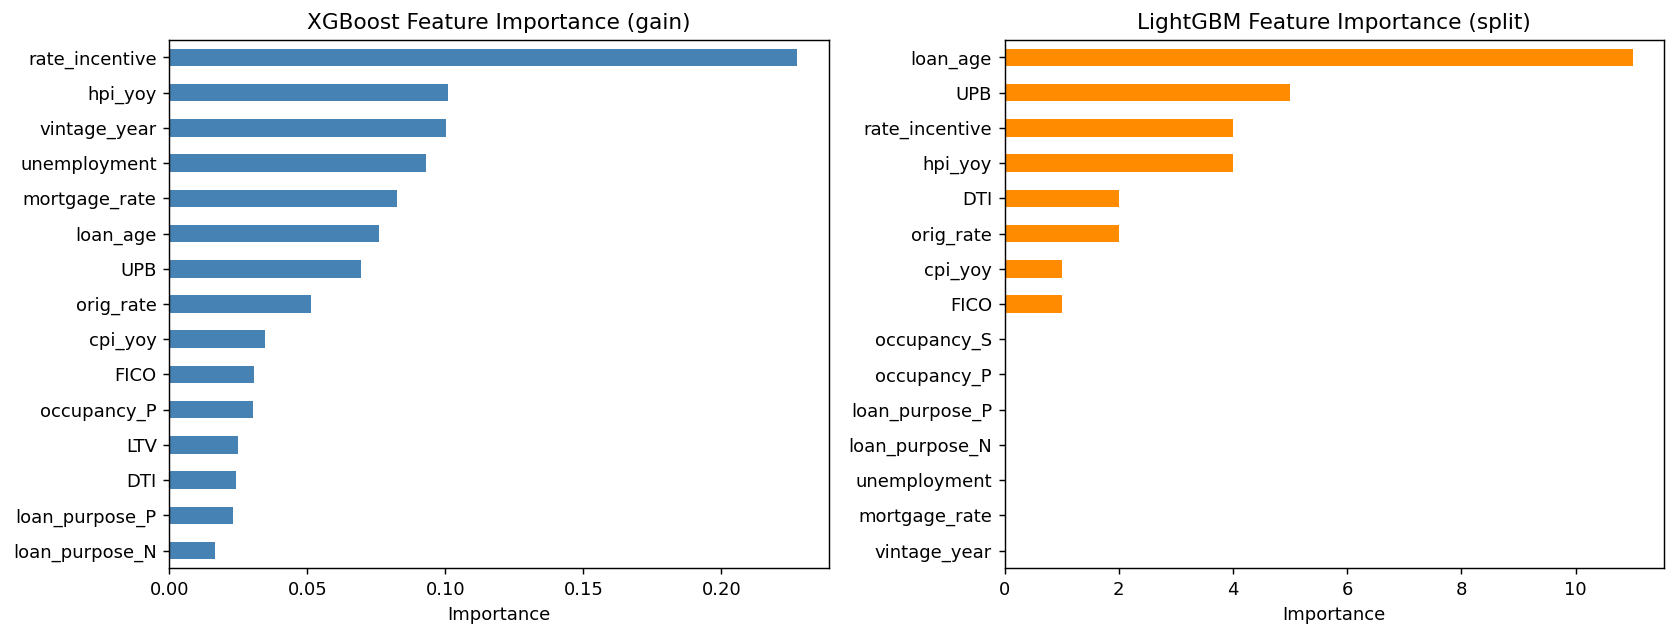
\includegraphics[width=\linewidth]{processed/C_feature_importance.png}
        \caption{\small Top features: XGBoost / LightGBM / Random Forest}
      \end{figure}
  \end{columns}
\end{frame}

% ══════════════════════════════════════════════════════════════════════════════
\section{Part D: Deep Cox Model}

\begin{frame}{Deep Cox — Architecture \& Training}
  \[
    \lambda(t \mid \mathbf{x}) \;=\; \lambda_0(t)\,\exp\!\bigl(f_\theta(\mathbf{x})\bigr),
    \qquad
    \mathcal{L}(\theta) = -\frac{1}{|\mathcal{E}|}\sum_{i\in\mathcal{E}}
    \Bigl[f_\theta(\mathbf{x}_i) - \log\!\sum_{j:T_j\ge T_i}e^{f_\theta(\mathbf{x}_j)}\Bigr]
  \]
  \begin{columns}
    \column{0.50\textwidth}
      \textbf{Architecture:} Input(10) $\to$ 256 $\to$ 128 $\to$ 64 $\to$ 1\\
      BatchNorm + ReLU + Dropout(0.3) per layer
      \vspace{0.3em}

      \textbf{Training setup:}
      \begin{itemize}\small
        \item 500K loans, sorted by descending duration
        \item Adam, lr $= 10^{-3}$, weight decay $10^{-4}$
        \item 40 epochs, batch size 4096
        \item \texttt{torch.device("mps")} — Apple M1 Neural Engine
      \end{itemize}
    \column{0.46\textwidth}
      \begin{figure}
        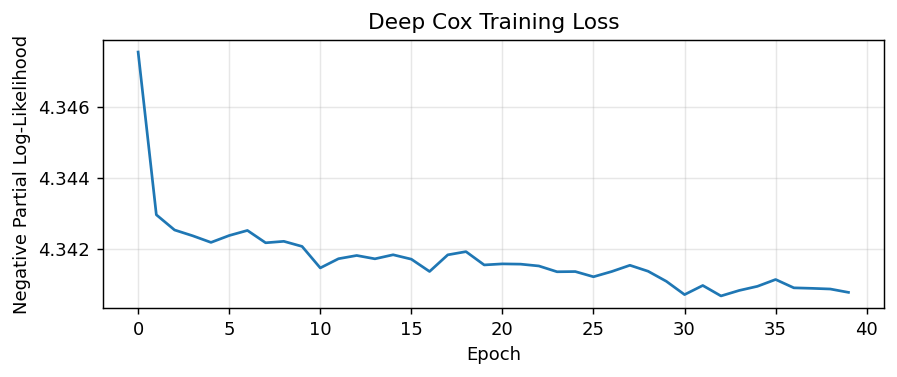
\includegraphics[width=\linewidth]{processed/D_training_loss.png}
        \caption{\small Negative partial log-likelihood over 40 epochs}
      \end{figure}
  \end{columns}
\end{frame}

\begin{frame}{Deep Cox — Does Nonlinearity Help?}
  \begin{columns}
    \column{0.50\textwidth}
      \begin{table}
        \small
        \begin{tabular}{lc}
          \toprule
          \textbf{Model} & \textbf{C-index} \\
          \midrule
          Cox PH (static)       & 0.611 \\
          LightGBM              & 0.672 \\
          \textbf{Deep Cox}     & \textbf{0.647} \\
          XGBoost               & 0.731 \\
          Elastic Net           & 0.798 \\
          \bottomrule
        \end{tabular}
        \caption{\small Test set. Deep Cox trained on 500K loan subsample.}
      \end{table}
      \vspace{0.3em}
      Deep Cox \textbf{improves on static Cox by +3.6 pp} in C-index,
      confirming nonlinear interactions matter.
    \column{0.46\textwidth}
      \begin{itemize}
        \item Deep Cox does not match tree models — likely because
          tree methods also capture time-varying macro context
          through the panel framing
        \item Deep Cox advantage: grounded in partial likelihood,
          gives well-defined risk scores, extends to time-varying inputs
        \item Nonlinear interactions (rate incentive $\times$ loan age,
          LTV $\times$ HPI) drive the gain over linear Cox
      \end{itemize}
      \begin{block}{Burnout via nonlinearity}
        The MLP implicitly captures diminishing hazard
        sensitivity at high loan ages.
      \end{block}
  \end{columns}
\end{frame}

\begin{frame}{Deep Cox — Gradient Sensitivity Analysis}
  \begin{columns}
    \column{0.52\textwidth}
      \begin{figure}
        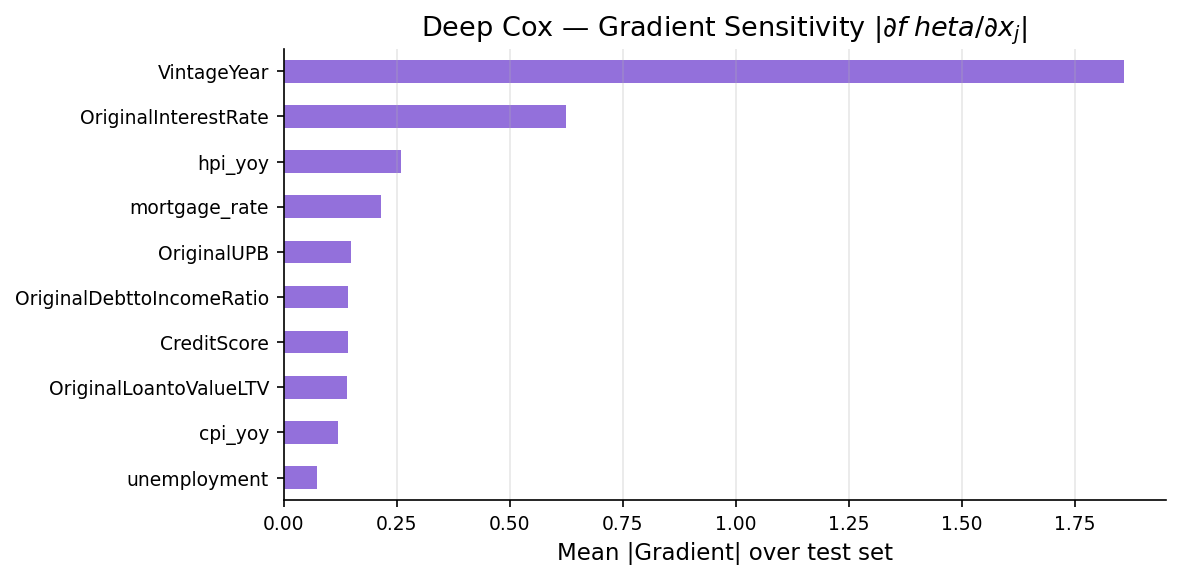
\includegraphics[width=\linewidth]{processed/D_gradient_sensitivity.png}
        \caption{\small Mean $|\partial f_\theta/\partial x_j|$ over test set}
      \end{figure}
    \column{0.44\textwidth}
      \textbf{Neural network analogue of hazard ratios.}\\[0.4em]
      Unlike Cox where $\partial f/\partial x_j = \beta_j$ is constant,
      the MLP gradient varies per loan — capturing interactions.
      \vspace{0.4em}
      \begin{itemize}\small
        \item \texttt{OriginalInterestRate} and \texttt{mortgage\_rate}
          dominate — consistent with refi-incentive theory
        \item \texttt{VintageYear} effect: recent vintages more censored,
          suppressing hazard in later cohorts
        \item \texttt{LTV} and \texttt{FICO} contribute nonlinearly:
          effect is stronger at the tails (high-LTV burnout,
          low-FICO credit lock-out)
      \end{itemize}
      \begin{alertblock}{Key insight}
        Gradient magnitudes differ from linear Cox coefficients,
        confirming the MLP captures interactions Cox cannot.
      \end{alertblock}
  \end{columns}
\end{frame}

% ══════════════════════════════════════════════════════════════════════════════
\section{Part E: Extensions}

\begin{frame}{Competing Risks — Prepayment vs.\ Default}
  \begin{columns}
    \column{0.52\textwidth}
      \begin{figure}
        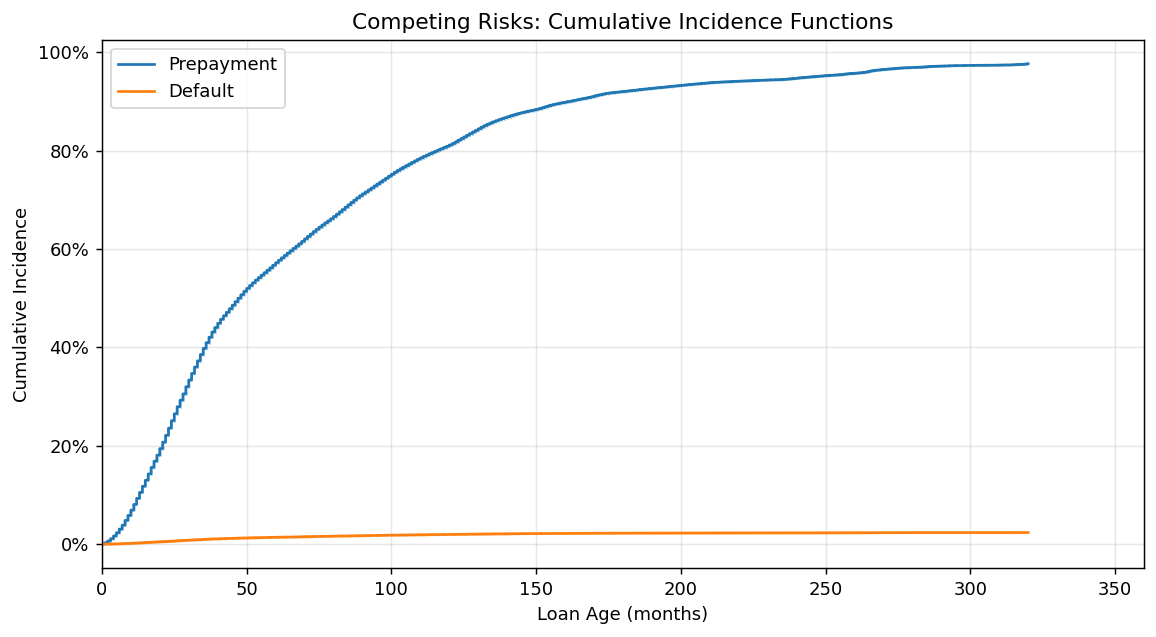
\includegraphics[width=\linewidth]{processed/E1_competing_risks_cif.png}
        \caption{\small Aalen-Johansen cumulative incidence functions}
      \end{figure}
    \column{0.44\textwidth}
      \textbf{10-year cumulative incidence:}
      \begin{itemize}
        \item Prepayment CIF: \textbf{81.1\%}
        \item Default CIF: \textbf{1.96\%}
      \end{itemize}
      \vspace{0.3em}
      KM \emph{overstates} prepayment probability by treating
      default as censoring rather than a competing absorbing state.
      \vspace{0.3em}
      \begin{itemize}
        \item Default risk concentrated in \textbf{2005–2008} vintages
          (peak: 9.4\% for 2007)
        \item Post-2012 defaults near zero — improved underwriting
          and rising home prices
        \item Risks are \alert{negatively correlated}: rate cuts
          trigger prepayment wave and suppress defaults simultaneously
      \end{itemize}
  \end{columns}
\end{frame}

\begin{frame}{Scenario Analysis — Rate Shock Sensitivity}
  \begin{columns}
    \column{0.54\textwidth}
      \begin{figure}
        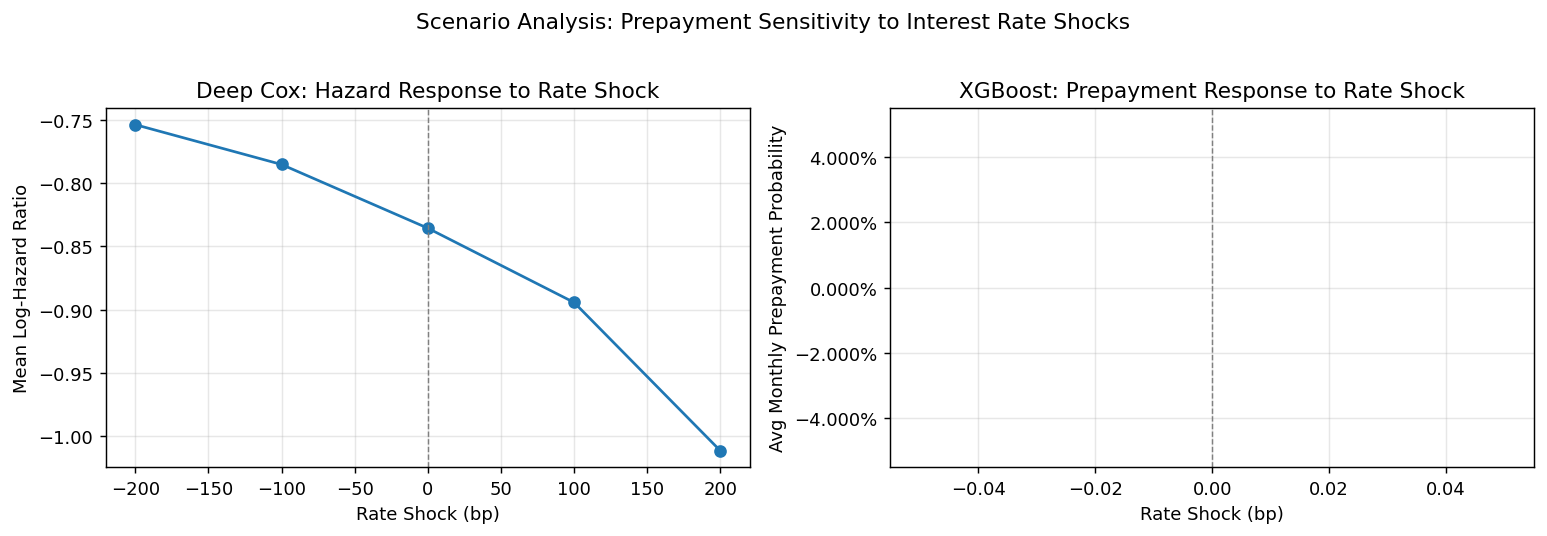
\includegraphics[width=\linewidth]{processed/E2_scenario_analysis.png}
        \caption{\small Prepayment response to parallel rate shocks}
      \end{figure}
    \column{0.42\textwidth}
      \textbf{Deep Cox log-hazard ratio vs.\ rate shock:}
      \begin{table}
        \small
        \begin{tabular}{rc}
          \toprule
          \textbf{Shock} & $\Delta\log\hat\lambda$ \\
          \midrule
          $-$200 bp & $+0.082$ \\
          $-$100 bp & $+0.051$ \\
          baseline  & 0 \\
          $+$100 bp & $-0.059$ \\
          $+$200 bp & $-0.176$ \\
          \bottomrule
        \end{tabular}
      \end{table}
      \vspace{0.2em}
      \small
      \textbf{Nonlinear response:} $-200$ bp raises hazard by 8.5\%
      but $+200$ bp lowers it by 16.1\% — asymmetric convexity
      consistent with borrower option theory.
  \end{columns}
\end{frame}

% ══════════════════════════════════════════════════════════════════════════════
\section{Conclusion}

\begin{frame}{Summary}
  \begin{columns}
    \column{0.48\textwidth}
      \textbf{What we built:}
      \begin{enumerate}
        \item[\textbf{A}] KM survival curves and hazard rates —
          seasoning hump at 24–48 months; burnout beyond 60
        \item[\textbf{B}] Cox PH + time-varying macro — PH violated
          for all key covariates; rate incentive dominates
        \item[\textbf{C}] XGBoost AUC 0.725 on 2020–22 backtest;
          Elastic Net C-index 0.798; Random Forest benchmarked
        \item[\textbf{D}] Deep Cox +3.6 pp over static Cox;
          gradient sensitivity confirms nonlinear interactions
        \item[\textbf{E}] Competing risks: 81\% prepay vs.\ 2\% default
          at 10 yr; asymmetric rate shock response
      \end{enumerate}
    \column{0.48\textwidth}
      \textbf{Key takeaways:}
      \begin{itemize}
        \item \alert{Rate incentive} is the dominant prepayment driver
          across all model families
        \item PH assumption \emph{strongly} violated —
          time-varying models are essential
        \item Tree-based ML best for prediction accuracy;
          Cox models better for interpretation
        \item Deep Cox bridges the gap: flexible yet
          grounded in survival theory
        \item Prepayment is \alert{convex} in rates —
          asymmetric MBS duration risk
      \end{itemize}
      \vspace{0.3em}
      \textbf{Future:} full MBS cash-flow Monte Carlo under
      rate path scenarios.
  \end{columns}
\end{frame}

\begin{frame}[plain]
  \begin{center}
    \Large\textbf{Thank you}\\[1em]
    \normalsize Questions?\\[2em]
    \small\texttt{yueqi.lin.baruchmfe@gmail.com}
  \end{center}
\end{frame}

% ══════════════════════════════════════════════════════════════════════════════
\appendix

\begin{frame}{Appendix — Data Pipeline}
  \small
  \begin{enumerate}
    \item \textbf{Origination} parquet files: filter \texttt{FRM + 360 months};
      34M qualifying loans (1999–2025).
    \item \textbf{Performance} parquet files: lazy Polars scan year-by-year;
      group by \texttt{LoanSequenceNumber}; extract first non-null
      \texttt{ZeroBalanceCode} as event (prepay = 1, default $\in\{2,3,9\}$)
      and corresponding \texttt{LoanAge}; censored = max observed age.
    \item \textbf{Join} origination $\bowtie$ performance $\Rightarrow$
      \texttt{survival\_loans.parquet} (293 MB, one row per loan).
    \item \textbf{ML panel}: stratified 2M-loan sample, expand to monthly
      rows, merge FRED macro by calendar month $\Rightarrow$
      \texttt{panel\_monthly.parquet} (193 MB).
  \end{enumerate}
\end{frame}

\begin{frame}{Appendix — Breslow Partial Likelihood}
  For data sorted by \textbf{descending} survival time:
  \[
    \mathcal{L}(\theta) = -\frac{1}{|\mathcal{E}|}
    \sum_{i \in \mathcal{E}}
    \Bigl[
      f_\theta(\mathbf{x}_i)
      - \log\!\sum_{j : T_j \geq T_i} \exp\!\bigl(f_\theta(\mathbf{x}_j)\bigr)
    \Bigr]
  \]
  Implemented via \texttt{torch.logcumsumexp} — $O(n)$ in a single forward pass.
  \vspace{0.5em}

  \textbf{Vintage breakdown highlights:}
  \begin{table}
    \small
    \begin{tabular}{lrcc}
      \toprule
      Vintage & Loans & Prepay rate & Default rate \\
      \midrule
      2006–2007 & 2.09M & 84.6\% & 8.9\% \\
      2012–2013 & 2.42M & 72.8\% & 0.8\% \\
      2020–2021 & 5.74M & 22.1\% & 0.0\% \\
      \bottomrule
    \end{tabular}
  \end{table}
\end{frame}

\end{document}
